% =============================================================================================
%  EpistemeGraph -- 6-page conference version (IEEE).  The full version is extended.tex.
%  Every quantitative result is a macro from generated/results.tex (scripts/export_paper_assets.py).
%  Overleaf: upload paper/EpistemeGraph_overleaf.zip (New Project -> Upload Project) and press Recompile.
% =============================================================================================
\documentclass[conference]{IEEEtran}
\IEEEoverridecommandlockouts

\usepackage[T1]{fontenc}
\usepackage[utf8]{inputenc}
\usepackage{cite}
\usepackage{amsmath,amssymb,amsthm,mathtools}
\usepackage{bm}
\usepackage{booktabs}
\usepackage{graphicx}
\usepackage{adjustbox}
\usepackage{xcolor}
\usepackage{microtype}
\usepackage[colorlinks=true,linkcolor=blue!50!black,citecolor=blue!50!black,urlcolor=blue!50!black]{hyperref}
\usepackage[capitalise,noabbrev]{cleveref}

\newtheorem{proposition}{Proposition}
\DeclareMathOperator{\logit}{logit}
\DeclareMathOperator{\spec}{spec}
\newcommand{\R}{\mathbb{R}}
\newcommand{\SKGq}{S_{\mathrm{KG}}(q)}

\IfFileExists{generated/results.tex}{% AUTO-GENERATED by scripts/export_paper_assets.py -- do not edit by hand
\newcommand{\SKG}{84.4}
\newcommand{\PhiProv}{86.8}
\newcommand{\PhiCov}{69.8}
\newcommand{\PhiTopo}{84.3}
\newcommand{\PhiCons}{99.5}
\newcommand{\NDocs}{3}
\newcommand{\NChunks}{76}
\newcommand{\NRawTriples}{613}
\newcommand{\NTriples}{375}
\newcommand{\NEntities}{313}
\newcommand{\NShared}{29}
\newcommand{\AcceptRate}{61.2}
\newcommand{\KGPrec}{53.0}
\newcommand{\KGPrecLo}{43.3}
\newcommand{\KGPrecHi}{62.5}
\newcommand{\KGPrecLenient}{85.0}
\newcommand{\KGAuditN}{100}
\newcommand{\KGAuditor}{claude-haiku-5-5}
\newcommand{\NItems}{400}
\newcommand{\NLabelled}{400}
\newcommand{\NTrain}{262}
\newcommand{\NCal}{65}
\newcommand{\NTest}{73}
\newcommand{\SupportedRate}{19.5}
\newcommand{\ExtentHal}{80.8}
\newcommand{\ExtentSup}{75.9}
\newcommand{\ExtentAUC}{0.511}
\newcommand{\Champion}{MonotoneHistGBM}
\newcommand{\TestAUC}{0.728}
\newcommand{\TestLL}{0.402}
\newcommand{\TestBrier}{0.123}
\newcommand{\TestECE}{0.054}
\newcommand{\TestAcc}{84.9}
\newcommand{\LLMAUC}{0.797}
\newcommand{\LLMECE}{0.324}
\newcommand{\Alpha}{0.10}
\newcommand{\Coverage}{97.3}
\newcommand{\CoverageSup}{92.3}
\newcommand{\CoverageHal}{98.3}
\newcommand{\AbstainRate}{76.7}
\newcommand{\SelAcc}{88.2}
\newcommand{\TauVer}{0.084}
\newcommand{\TauHal}{0.313}
\newcommand{\PoolBzero}{4.07}
\newcommand{\PoolBq}{0.98}
\newcommand{\PoolBkg}{-1.23}
\newcommand{\JudgeKappa}{--}
\newcommand{\JudgeN}{--}
\newcommand{\PrimaryJudge}{claude-sonnet-5-5}
\newcommand{\CrossJudge}{claude-haiku-5-5}
\newcommand{\CrossJudgeN}{100}
\newcommand{\CrossJudgeKappa}{0.35}
\newcommand{\CrossJudgeAgree}{80.0}
\newcommand{\TestAUCLo}{0.562}
\newcommand{\TestAUCHi}{0.870}
\newcommand{\LLMAUCLo}{0.612}
\newcommand{\LLMAUCHi}{0.927}
\newcommand{\DeltaLLM}{-0.069}
\newcommand{\PvalLLM}{0.492}
\newcommand{\DeltaText}{0.032}
\newcommand{\PvalText}{0.774}
\newcommand{\DeltaTopo}{0.010}
\newcommand{\PvalTopo}{0.797}
\newcommand{\KGAccLearned}{54.1}
\newcommand{\KGAccLo}{45.6}
\newcommand{\KGAccHi}{62.6}
\newcommand{\SensDefault}{0.8446}
\newcommand{\SensMaxDev}{0.0342}
\newcommand{\SensRange}{0.0557}
\newcommand{\AnswerModel}{claude-haiku-5-5}
\newcommand{\JudgeModel}{claude-sonnet-5-5}
\newcommand{\CVProtocol}{5x5 repeated stratified CV, n=400}
\newcommand{\CVAUC}{0.742}
\newcommand{\CVAUCsd}{0.052}
\newcommand{\CVAUCLo}{0.633}
\newcommand{\CVAUCHi}{0.780}
\newcommand{\CVAUCvthree}{0.737}
\newcommand{\CVAUCtext}{0.705}
\newcommand{\CVAUCllm}{0.591}
\newcommand{\CVAUClen}{0.628}
\newcommand{\CVECE}{0.090}
\newcommand{\CVECEllm}{0.342}
\newcommand{\CVPvthree}{0.588}
\newcommand{\CVPllm}{0.022}
\newcommand{\CVPtext}{0.876}
\newcommand{\CVPlen}{0.049}
\newcommand{\SevereAUC}{0.708}
\newcommand{\SevereLLM}{0.662}
\newcommand{\SevereN}{300}
\newcommand{\VthreeTestAUC}{0.671}
\newcommand{\VthreeChampion}{RandomForest}
\newcommand{\KappaUnsup}{0.48}
\newcommand{\KappaOrd}{0.41}
\newcommand{\AUCvsSecond}{0.714}
\newcommand{\AUCvsPrimarySame}{0.723}
\newcommand{\AUCagree}{0.756}
\newcommand{\NAgree}{80}
\newcommand{\LenAUC}{0.604}
\newcommand{\FPAccepted}{38.8}
\newcommand{\NPartial}{222}
\newcommand{\NUnsup}{100}
\newcommand{\NSup}{78}
\newcommand{\CostRun}{1.90}
\newcommand{\KappaFull}{0.57}
\newcommand{\AgreeFull}{87.2}
\newcommand{\ConsensusN}{349}
\newcommand{\ConsensusAUC}{0.762}
\newcommand{\ConsensusLLM}{0.571}
\newcommand{\ConsensusMatched}{305}
\newcommand{\GeminiName}{Gemini Pro (high reasoning)}
\newcommand{\GeminiSupp}{70.0}
\newcommand{\GeminiKappa}{0.17}
\newcommand{\GeminiAUC}{0.486}
\newcommand{\GeminiLLMAUC}{0.714}
\newcommand{\MajorityAUC}{0.727}
\newcommand{\MajorityLLMAUC}{0.650}
\newcommand{\NUnanimous}{32}
\newcommand{\ThirdJudgeSentence}{A third judge from a different model family (\texttt{Gemini Pro (high reasoning)}), given the three papers in full and blind to the other verdicts, labelled the same 100 answers; its binary agreement with the primary judge is $\kappa=0.17$ (raw agreement 49.0\%).}
\newcommand{\HumanJudgeSentence}{}
\newcommand{\HaikuLabelCVAUC}{0.736}
\newcommand{\HaikuLabelCVAUCllm}{0.548}
\newcommand{\HaikuLabelCVAUCvthree}{0.697}
\newcommand{\CatCrossLLM}{0.219}
\newcommand{\CatFPLLM}{0.709}
\newcommand{\HKvsSonnet}{0.797}
\newcommand{\HKvsHaiku}{0.722}
\newcommand{\HaikuLabelKappa}{0.35}
\newcommand{\MatchN}{330}
\newcommand{\MatchTotal}{400}
\newcommand{\MatchBase}{322}
\newcommand{\BalAcc}{62.9}
\newcommand{\Committed}{137}
\newcommand{\CommittedCorrect}{114}
\newcommand{\KGPrecLenientLo}{76.7}
\newcommand{\KGPrecLenientHi}{90.7}
\newcommand{\KGNIncorrect}{15}
\newcommand{\KGNPartial}{32}
\newcommand{\CVCovTen}{94.2}
\newcommand{\CVAbsTen}{65.8}
\newcommand{\CVSelTen}{83.0}
\newcommand{\CVAbsTwenty}{48.8}
\newcommand{\CVSelTwenty}{83.1}
\newcommand{\PoolLRTp}{0.040}
\newcommand{\PoolLRTchi}{4.22}
\newcommand{\PoolKGused}{kept}
\newcommand{\CatBorderLLM}{0.341}
\newcommand{\CatBorderLen}{0.752}
\newcommand{\CatBorderVfour}{0.685}
\newcommand{\CatCrossVfour}{0.539}
\newcommand{\CatCrossVthree}{0.664}
\newcommand{\CatFactLLM}{0.759}
\newcommand{\CatFactVfour}{0.695}
\newcommand{\CatFPVfour}{0.776}
\newcommand{\PoolCVwith}{0.4494}
\newcommand{\PoolCVwithout}{0.4506}
\newcommand{\TestAUCq}{0.746}
\newcommand{\AUCvsSecondLLM}{0.395}
\newcommand{\OrdAUC}{0.739}
\newcommand{\BinAUC}{0.734}

\newcommand{\TableCv}{%
\begin{table}[t]\centering\footnotesize
\caption{Repeated cross-validation over all labelled answers (\CVProtocol). Pooled out-of-fold AUROC, mean $\pm$ s.d. over folds, 95\% bootstrap CI and ECE of one repetition, and the paired DeLong $p$-value against EpistemeGraph v4.}\label{tab:cv}
\begin{adjustbox}{max width=\columnwidth}\begin{tabular}{lccccc}\toprule
Detector & AUROC & fold mean $\pm$ s.d. & 95\% CI & ECE & $p$ (DeLong) \\ \midrule
\textbf{EpistemeGraph} & 0.742 & 0.741 $\pm$ 0.052 & [0.633, 0.780] & 0.090 & -- \\
Same learner, 13 answer features & 0.737 & 0.741 $\pm$ 0.066 & [0.659, 0.792] & 0.079 & $0.588$ \\
Text-only NLI checker & 0.705 & 0.708 $\pm$ 0.068 & [0.640, 0.776] & 0.027 & $0.876$ \\
LLM verbalised confidence & 0.591 & 0.591 $\pm$ 0.076 & [0.504, 0.677] & 0.342 & $0.022$ \\
Answer length & 0.628 & 0.634 $\pm$ 0.078 & [0.551, 0.702] & 0.042 & $0.049$ \\
\bottomrule\end{tabular}\end{adjustbox}
\end{table}}

\newcommand{\TableConformal}{%
\begin{table}[t]\centering\footnotesize
\caption{Risk--abstention trade-off of the Mondrian cross-conformal decision over all labelled answers (out-of-fold scores, 5-fold calibration).}\label{tab:conformal}
\begin{adjustbox}{max width=\columnwidth}\begin{tabular}{cccccc}\toprule
$\alpha$ & Coverage & Cov.\ sup. & Cov.\ hal. & Abstain & Sel.\ acc. \\ \midrule
0.05 & 95.8 & 96.2 & 95.7 & 82.2 & 76.5 \\
0.10 & 94.2 & 91.2 & 95.0 & 65.8 & 83.0 \\
0.15 & 93.2 & 86.2 & 95.0 & 60.5 & 82.7 \\
0.20 & 91.5 & 77.3 & 95.0 & 48.8 & 83.1 \\
0.25 & 91.2 & 76.1 & 95.0 & 41.0 & 85.4 \\
0.30 & 90.5 & 72.2 & 95.0 & 38.5 & 84.8 \\
\bottomrule\end{tabular}\end{adjustbox}
\end{table}}

\newcommand{\TableClaimimp}{%
\begin{table}[t]\centering\footnotesize
\caption{Grouped permutation importance of the pooled claim statistics (mean, min, max of one claim feature permuted jointly; increase in test log-loss).}\label{tab:claimimp}
\begin{adjustbox}{max width=\columnwidth}\begin{tabular}{lcc}\toprule
Claim feature & $\Delta$ log-loss & s.d. \\ \midrule
NLI contradiction & 0.0097 & 0.0155 \\
NLI entailment & 0.0079 & 0.0063 \\
Out-of-corpus rate & 0.0053 & 0.0031 \\
Grafted-edge curvature & 0.0053 & 0.0044 \\
Provenance strength & 0.0044 & 0.0048 \\
Evidence similarity & 0.0019 & 0.0024 \\
Sheaf residual & 0.0017 & 0.0033 \\
Two-hop KG path & 0.0015 & 0.0007 \\
Speculative polarity & 0.0013 & 0.0012 \\
Entity alignment & 0.0012 & 0.0017 \\
Refuted polarity & 0.0002 & 0.0006 \\
Conflict flag & 0.0000 & 0.0000 \\
Asserted polarity & -0.0013 & 0.0014 \\
Direct KG edge & -0.0017 & 0.0040 \\
NLI consistency & -0.0085 & 0.0061 \\
\bottomrule\end{tabular}\end{adjustbox}
\end{table}}

\newcommand{\TableLeaderboard}{%
\begin{table}[t]\centering\footnotesize
\caption{Ten-model tournament (nested 5$\times$3 CV on the training split, out-of-fold metrics). $^\star$ marks the champion, selected by log-loss.}\label{tab:leaderboard}
\begin{adjustbox}{max width=\columnwidth}\begin{tabular}{lcccc}\toprule
Model & Log-loss$\downarrow$ & AUROC$\uparrow$ & Brier$\downarrow$ & ECE$\downarrow$ \\ \midrule
Monotone gradient boosting$^\star$ & 0.373 & 0.809 & 0.117 & 0.062 \\
Gradient boosting & 0.376 & 0.807 & 0.116 & 0.041 \\
Stacking ensemble & 0.388 & 0.774 & 0.117 & 0.040 \\
Random forest & 0.397 & 0.768 & 0.121 & 0.069 \\
RBF-kernel SVM & 0.405 & 0.767 & 0.124 & 0.034 \\
Extra trees & 0.416 & 0.756 & 0.129 & 0.044 \\
Logistic regression & 0.418 & 0.720 & 0.127 & 0.037 \\
Attention MIL network & 0.495 & 0.562 & 0.149 & 0.051 \\
Multilayer perceptron & 0.573 & 0.438 & 0.189 & 0.175 \\
Attention ResNet & 0.621 & 0.632 & 0.209 & 0.221 \\
\bottomrule\end{tabular}\end{adjustbox}
\end{table}}

\newcommand{\TableAblation}{%
\begin{table}[t]\centering\footnotesize
\caption{Feature-family ablation (standardised logistic model, held-out test split; 95\% bootstrap CI).}\label{tab:ablation}
\begin{adjustbox}{max width=\columnwidth}\begin{tabular}{lcccc}\toprule
Feature set & AUROC & 95\% CI & Log-loss & ECE \\ \midrule
All inputs & 0.731 & [0.559, 0.867] & 0.450 & 0.111 \\
13 answer features only & 0.763 & [0.608, 0.888] & 0.403 & 0.119 \\
Pooled claims only & 0.638 & [0.444, 0.811] & 0.470 & 0.128 \\
Topological only & 0.631 & [0.439, 0.796] & 0.446 & 0.095 \\
Evidential only & 0.637 & [0.415, 0.830] & 0.455 & 0.112 \\
Model signals only & 0.758 & [0.583, 0.920] & 0.395 & 0.120 \\
Text NLI only & 0.696 & [0.511, 0.854] & 0.426 & 0.078 \\
Graph only & 0.650 & [0.445, 0.814] & 0.449 & 0.103 \\
Without topological & 0.721 & [0.530, 0.886] & 0.418 & 0.042 \\
Without model signals & 0.651 & [0.469, 0.826] & 0.481 & 0.101 \\
\bottomrule\end{tabular}\end{adjustbox}
\end{table}}

\newcommand{\TableSens}{%
\begin{table}[t]\centering\footnotesize
\caption{Phase 1 robustness: every design constant perturbed one at a time and the pipeline re-run on the cached extractions (no API calls).}\label{tab:sens}
\begin{adjustbox}{max width=\columnwidth}\begin{tabular}{lccccccc}\toprule
Constant & Value & $S_{\mathrm{KG}}$ & $\Phi_{\mathrm{prov}}$ & $\Phi_{\mathrm{cov}}$ & $\Phi_{\mathrm{topo}}$ & Triples & Entities \\ \midrule
all defaults & -- & 0.8446 & 0.869 & 0.698 & 0.843 & 375 & 313 \\
verbatim quote-match ratio & 0.75 & 0.8446 & 0.869 & 0.698 & 0.843 & 375 & 313 \\
verbatim quote-match ratio & 0.9 & 0.8446 & 0.869 & 0.698 & 0.843 & 375 & 313 \\
entity support in the quote & 0.75 & 0.8788 & 0.869 & 0.771 & 0.897 & 552 & 408 \\
entity support in the quote & 0.95 & 0.8446 & 0.869 & 0.698 & 0.843 & 375 & 313 \\
coverage normaliser tau & 0.5 & 0.8649 & 0.869 & 0.768 & 0.843 & 375 & 313 \\
coverage normaliser tau & 0.7 & 0.8231 & 0.869 & 0.630 & 0.843 & 375 & 313 \\
min. extractor confidence & 0.3 & 0.8443 & 0.868 & 0.698 & 0.843 & 375 & 313 \\
min. extractor confidence & 0.7 & 0.8453 & 0.871 & 0.697 & 0.845 & 374 & 311 \\
entity-merge cosine & 0.8 & 0.8486 & 0.869 & 0.697 & 0.861 & 374 & 295 \\
entity-merge cosine & 0.9 & 0.8454 & 0.869 & 0.701 & 0.842 & 381 & 324 \\
\bottomrule\end{tabular}\end{adjustbox}
\end{table}}

\newcommand{\TableTripleweights}{%
\begin{table}[t]\centering\footnotesize
\caption{Learned weights of the triple-correctness model used by the model-assisted KG-accuracy estimator (standardised logistic coefficients).}\label{tab:tripleweights}
\begin{adjustbox}{max width=\columnwidth}\begin{tabular}{lc}\toprule
Evidence signal & Weight \\ \midrule
extraction confidence & 0.69 \\
log quote len & 0.45 \\
grounding score & 0.30 \\
log support & 0.20 \\
cross pdf & -0.03 \\
log relation freq & -0.11 \\
log deg object & -0.17 \\
log deg subject & -0.27 \\
verbatim & -0.37 \\
\bottomrule\end{tabular}\end{adjustbox}
\end{table}}

\newcommand{\TableFeatures}{%
\begin{table}[t]\centering\footnotesize
\caption{Individual features: sign-oriented single-feature AUROC on the test split, learned standardised weight $w_j$ and permutation importance of the champion.}\label{tab:features}
\begin{adjustbox}{max width=\columnwidth}\begin{tabular}{lllccc}\toprule
 & Feature & Family & AUROC & $w_j$ & Perm. imp. \\ \midrule
$\mathcal{E}_{\mathcal{F}}$ & Sheaf Laplacian energy & topological & 0.382 & 0.37 & 0.000 \\
$\Delta\kappa$ & Forman-Ricci curvature shift & topological & 0.717 & -0.19 & 0.016 \\
$D_{\mathrm{spec}}$ & Spectral Wasserstein divergence & topological & 0.469 & -0.10 & -0.004 \\
$\pi_{\mathrm{prov}}$ & Bayesian provenance support & evidential & 0.569 & 0.25 & 0.000 \\
$\sigma_{\mathrm{sim}}$ & Evidence embedding similarity & evidential & 0.447 & -0.21 & 0.002 \\
$\bar\gamma_{\mathrm{NLI}}$ & Mean NLI consistency (SummaC-ZS) & evidential & 0.463 & -0.16 & 0.008 \\
$\gamma^{\min}_{\mathrm{NLI}}$ & Worst-claim NLI consistency & evidential & 0.556 & 0.31 & 0.002 \\
$\nu_{\mathrm{ooc}}$ & Out-of-corpus novelty (IDF) & evidential & 0.439 & 0.17 & 0.000 \\
$\kappa_{\mathrm{con}}$ & Graph contradiction rate & evidential & 0.501 & 0.24 & 0.000 \\
$\rho_{\mathrm{align}}$ & Entity alignment rate & evidential & 0.466 & 0.34 & -0.003 \\
$c_{\mathrm{LLM}}$ & LLM verbalised confidence & model & 0.797 & 0.21 & 0.031 \\
$\bar u_{\mathrm{NLL}}$ & Mean token negative log-likelihood & model & 0.500 & 0.00 & 0.000 \\
$h_{\mathrm{spec}}$ & Speculative-claim ratio & model & 0.500 & -0.05 & 0.000 \\
\bottomrule\end{tabular}\end{adjustbox}
\end{table}}

\newcommand{\TablePercat}{%
\begin{table}[t]\centering\footnotesize
\caption{Per-category behaviour on the test split ($\alpha=\Alpha$).}\label{tab:percat}
\begin{adjustbox}{max width=\columnwidth}\begin{tabular}{lcccccc}\toprule
Category & $n$ & Supported \% & mean $S_{\text{final}}$ & VER & ABS & HAL \\ \midrule
BORDERLINE & 13 & 7.7 & 0.235 & 1 & 10 & 2 \\
CROSS\_DOC & 10 & 10.0 & 0.190 & 0 & 9 & 1 \\
FACTUAL & 26 & 26.9 & 0.160 & 0 & 18 & 8 \\
FALSE\_PREMISE & 24 & 16.7 & 0.260 & 3 & 19 & 2 \\
\bottomrule\end{tabular}\end{adjustbox}
\end{table}}

\newcommand{\TableKgprec}{%
\begin{table}[t]\centering\footnotesize
\caption{Extrinsic KG precision per source paper (strict, 95\% Wilson interval; lenient counts partially correct triples as correct).}\label{tab:kgprec}
\begin{adjustbox}{max width=\columnwidth}\begin{tabular}{lcccc}\toprule
Paper & $n$ & Precision & 95\% CI & Lenient \\ \midrule
paper1.pdf & 39 & 46.2 & [31.6, 61.4] & 82.1 \\
paper2.pdf & 33 & 60.6 & [43.7, 75.3] & 87.9 \\
paper3.pdf & 28 & 53.6 & [35.8, 70.5] & 85.7 \\
\bottomrule\end{tabular}\end{adjustbox}
\end{table}}
}{% AUTO-GENERATED placeholders: every result macro renders as --
\providecommand{\SKG}{--}
\providecommand{\PhiProv}{--}
\providecommand{\PhiCov}{--}
\providecommand{\PhiTopo}{--}
\providecommand{\PhiCons}{--}
\providecommand{\NDocs}{--}
\providecommand{\NChunks}{--}
\providecommand{\NRawTriples}{--}
\providecommand{\NTriples}{--}
\providecommand{\NEntities}{--}
\providecommand{\NShared}{--}
\providecommand{\AcceptRate}{--}
\providecommand{\KGPrec}{--}
\providecommand{\KGPrecLo}{--}
\providecommand{\KGPrecHi}{--}
\providecommand{\KGPrecLenient}{--}
\providecommand{\KGAuditN}{--}
\providecommand{\KGAuditor}{--}
\providecommand{\NItems}{--}
\providecommand{\NLabelled}{--}
\providecommand{\NTrain}{--}
\providecommand{\NCal}{--}
\providecommand{\NTest}{--}
\providecommand{\SupportedRate}{--}
\providecommand{\ExtentHal}{--}
\providecommand{\ExtentSup}{--}
\providecommand{\ExtentAUC}{--}
\providecommand{\Champion}{--}
\providecommand{\TestAUC}{--}
\providecommand{\TestLL}{--}
\providecommand{\TestBrier}{--}
\providecommand{\TestECE}{--}
\providecommand{\TestAcc}{--}
\providecommand{\LLMAUC}{--}
\providecommand{\LLMECE}{--}
\providecommand{\Alpha}{--}
\providecommand{\Coverage}{--}
\providecommand{\CoverageSup}{--}
\providecommand{\CoverageHal}{--}
\providecommand{\AbstainRate}{--}
\providecommand{\SelAcc}{--}
\providecommand{\TauVer}{--}
\providecommand{\TauHal}{--}
\providecommand{\PoolBzero}{--}
\providecommand{\PoolBq}{--}
\providecommand{\PoolBkg}{--}
\providecommand{\JudgeKappa}{--}
\providecommand{\JudgeN}{--}
\providecommand{\PrimaryJudge}{--}
\providecommand{\CrossJudge}{--}
\providecommand{\CrossJudgeN}{--}
\providecommand{\CrossJudgeKappa}{--}
\providecommand{\CrossJudgeAgree}{--}
\providecommand{\TestAUCLo}{--}
\providecommand{\TestAUCHi}{--}
\providecommand{\LLMAUCLo}{--}
\providecommand{\LLMAUCHi}{--}
\providecommand{\DeltaLLM}{--}
\providecommand{\PvalLLM}{--}
\providecommand{\DeltaText}{--}
\providecommand{\PvalText}{--}
\providecommand{\DeltaTopo}{--}
\providecommand{\PvalTopo}{--}
\providecommand{\KGAccLearned}{--}
\providecommand{\KGAccLo}{--}
\providecommand{\KGAccHi}{--}
\providecommand{\SensDefault}{--}
\providecommand{\SensMaxDev}{--}
\providecommand{\SensRange}{--}
\providecommand{\AnswerModel}{--}
\providecommand{\JudgeModel}{--}
\providecommand{\CVProtocol}{--}
\providecommand{\CVAUC}{--}
\providecommand{\CVAUCsd}{--}
\providecommand{\CVAUCLo}{--}
\providecommand{\CVAUCHi}{--}
\providecommand{\CVAUCvthree}{--}
\providecommand{\CVAUCtext}{--}
\providecommand{\CVAUCllm}{--}
\providecommand{\CVAUClen}{--}
\providecommand{\CVECE}{--}
\providecommand{\CVECEllm}{--}
\providecommand{\CVPvthree}{--}
\providecommand{\CVPllm}{--}
\providecommand{\CVPtext}{--}
\providecommand{\CVPlen}{--}
\providecommand{\SevereAUC}{--}
\providecommand{\SevereLLM}{--}
\providecommand{\SevereN}{--}
\providecommand{\VthreeTestAUC}{--}
\providecommand{\VthreeChampion}{--}
\providecommand{\KappaUnsup}{--}
\providecommand{\KappaOrd}{--}
\providecommand{\AUCvsSecond}{--}
\providecommand{\AUCvsPrimarySame}{--}
\providecommand{\AUCagree}{--}
\providecommand{\NAgree}{--}
\providecommand{\LenAUC}{--}
\providecommand{\FPAccepted}{--}
\providecommand{\NPartial}{--}
\providecommand{\NUnsup}{--}
\providecommand{\NSup}{--}
\providecommand{\CostRun}{--}
\providecommand{\KappaFull}{--}
\providecommand{\AgreeFull}{--}
\providecommand{\ConsensusN}{--}
\providecommand{\ConsensusAUC}{--}
\providecommand{\ConsensusLLM}{--}
\providecommand{\ConsensusMatched}{--}
\providecommand{\GeminiName}{--}
\providecommand{\GeminiSupp}{--}
\providecommand{\GeminiKappa}{--}
\providecommand{\GeminiAUC}{--}
\providecommand{\GeminiLLMAUC}{--}
\providecommand{\MajorityAUC}{--}
\providecommand{\MajorityLLMAUC}{--}
\providecommand{\NUnanimous}{--}
\providecommand{\ThirdJudgeSentence}{}
\providecommand{\HumanJudgeSentence}{}
\providecommand{\HaikuLabelCVAUC}{--}
\providecommand{\HaikuLabelCVAUCllm}{--}
\providecommand{\HaikuLabelCVAUCvthree}{--}
\providecommand{\CatCrossLLM}{--}
\providecommand{\CatFPLLM}{--}
\providecommand{\HKvsSonnet}{--}
\providecommand{\HKvsHaiku}{--}
\providecommand{\HaikuLabelKappa}{--}
\providecommand{\MatchN}{--}
\providecommand{\MatchTotal}{--}
\providecommand{\MatchBase}{--}
\providecommand{\BalAcc}{--}
\providecommand{\Committed}{--}
\providecommand{\CommittedCorrect}{--}
\providecommand{\KGPrecLenientLo}{--}
\providecommand{\KGPrecLenientHi}{--}
\providecommand{\KGNIncorrect}{--}
\providecommand{\KGNPartial}{--}
\providecommand{\CVCovTen}{--}
\providecommand{\CVAbsTen}{--}
\providecommand{\CVSelTen}{--}
\providecommand{\CVAbsTwenty}{--}
\providecommand{\CVSelTwenty}{--}
\providecommand{\PoolLRTp}{--}
\providecommand{\PoolLRTchi}{--}
\providecommand{\PoolKGused}{--}
\providecommand{\CatBorderLLM}{--}
\providecommand{\CatBorderLen}{--}
\providecommand{\CatBorderVfour}{--}
\providecommand{\CatCrossVfour}{--}
\providecommand{\CatCrossVthree}{--}
\providecommand{\CatFactLLM}{--}
\providecommand{\CatFactVfour}{--}
\providecommand{\CatFPVfour}{--}
\providecommand{\PoolCVwith}{--}
\providecommand{\PoolCVwithout}{--}
\providecommand{\TestAUCq}{--}
\providecommand{\AUCvsSecondLLM}{--}
\providecommand{\OrdAUC}{--}
\providecommand{\BinAUC}{--}
\providecommand{\TableCv}{}
\providecommand{\TableConformal}{}
\providecommand{\TableClaimimp}{}
\providecommand{\TableLeaderboard}{}
\providecommand{\TableAblation}{}
\providecommand{\TableSens}{}
\providecommand{\TableTripleweights}{}
\providecommand{\TableFeatures}{}
\providecommand{\TablePercat}{}
\providecommand{\TableKgprec}{}
}

\begin{document}

\title{EpistemeGraph: Auditing LLM Answers Against a Measured Knowledge Graph with Geometric Claim Evidence and Cross-Conformal Decisions}

\author{\IEEEauthorblockN{Anurag Raj}
\IEEEauthorblockA{\textit{Department of Computer Science and Engineering}\\
\textit{Indian Institute of Technology Ropar}\\
\texttt{rajanurag1508@gmail.com}\quad \url{https://github.com/Virtuoso-8051/EpistemeGraph}}}

\maketitle

\begin{abstract}
Large language models answer questions about specialised literature fluently and confidently even when they
misattribute results, invent details or accept a false premise. We present \emph{EpistemeGraph}, an auditor that
decides whether an answer is supported by a document collection, with what probability, how much of it is unsupported
and which claims are at fault. It builds a provenance-verified knowledge graph (KG) from the PDFs and measures its
precision, extracts the answer's claim graph in a call decoupled from generation, and describes every claim with
natural-language inference against source sentences and with graph geometry (sheaf energy, Forman--Ricci curvature of
the grafted edge, spectral divergence). A ten-model tournament under a proper scoring rule, cross-fitted calibration
and Mondrian cross-conformal prediction turn these measurements into \textsc{verified}, \textsc{abstain} or
\textsc{hallucinated} decisions with no hand-set weight or threshold. On \NItems{} questions over the DeepWalk, LINE and
node2vec papers, answered closed-book by \texttt{\AnswerModel}, the audit reaches AUROC \CVAUC{} in repeated
cross-validation, against \CVAUCllm{} for the model's own confidence ($p=\CVPllm$), and \ConsensusAUC{} on the answers
where two judges agree. Auditing the labels shows that judges agree only moderately ($\kappa=\KappaFull$) and that a
judge from another model family applies a far more lenient notion of support ($\kappa=\GeminiKappa$), which bounds every
metric. The study cost \$\CostRun{} in API calls; code and data are public.
\end{abstract}

\begin{IEEEkeywords}
hallucination detection, knowledge graphs, sheaf Laplacian, Ricci curvature, conformal prediction, LLM-as-a-judge
\end{IEEEkeywords}

\section{Introduction}
Hallucination, content that is fluent but unsupported by the relevant source, is the central obstacle to deploying LLMs
in technical domains~\cite{ji2023survey,huang2025survey}. A model's verbalised confidence is a weak signal on specialised
material~\cite{xiong2024uncertainty,kadavath2022know,tian2023just}, and text-to-text checkers cannot always separate a
claim that \emph{uses} the corpus vocabulary from one that is \emph{supported} by it: ``node2vec optimises a genetic
fitness function'' shares many tokens with the node2vec paper and is still false. Knowledge graphs offer a structured
alternative~\cite{kim2023factkg,sansford2024grapheval}, but raise four questions we address: how accurate is an
LLM-built reference graph, \emph{measured} rather than assumed; which quantities expose an unsupported claim; how can
many signals become a decision with a stated error rate and no hand-tuned weight; and how reliable are the labels
against which all of this is scored?

\paragraph*{Contributions}
(i)~A measured reference graph: provenance-verified KG construction, a fidelity index whose aggregation is derived
(\cref{prop:gm}) and an extrinsic precision audit. (ii)~Claim-level evidence combining NLI with knowledge-sheaf
residuals and grafted-edge curvature, and a permutation-invariant claim-set representation (\cref{prop:mi}).
(iii)~A fully learned, cross-fitted decision layer in which reference reliability must pass two statistical checks
(\cref{prop:pool}) and conformal verdicts never contradict their probability. (iv)~A label-audited evaluation with three
judges, a length confound and repeated cross-validation, reporting negative results where they occur.

\section{Related Work}
Reference-free detectors use sampling consistency~\cite{manakul2023selfcheckgpt}, semantic
entropy~\cite{farquhar2024semantic} or elicited confidence~\cite{kadavath2022know,tian2023just}; reference-based ones
verify atomic facts against a source~\cite{min2023factscore}. RAGTruth~\cite{niu2024ragtruth} fixed the convention, which
we follow, that a response is hallucinated if it contains any unsupported content. FactKG~\cite{kim2023factkg} and
GraphEval~\cite{sansford2024grapheval} verify claims against a KG; we additionally measure the KG, use graph geometry and
attach a distribution-free guarantee. The instruments are established: knowledge
sheaves~\cite{hansen2019sheaves,gebhart2023knowledge} with TransE as a special case~\cite{bordes2013transe}, Forman
curvature~\cite{forman2003bochner,samal2018comparative}, Laplacian spectra~\cite{chung1997spectral}, NLI
consistency~\cite{laban2022summac}, multiple-instance learning~\cite{dietterich1997mil,ilse2018attention}, Deep
Sets~\cite{zaheer2017deepsets}, proper scoring rules and calibration~\cite{gneiting2007scoring,platt1999probabilistic},
and Mondrian and cross-conformal prediction~\cite{vovk2012conditional,vovk2015cross,barber2021jackknife,angelopoulos2023gentle}.
LLM judges~\cite{zheng2023judging} show verbosity biases~\cite{dubois2024length}; we measure their agreement with Cohen's
$\kappa$~\cite{cohen1960kappa,landis1977measurement}.

\section{Method}
An answer $a$ to query $q$ is \emph{supported} ($y=1$) if every claim it asserts is stated in or entailed by the
documents (correctly rejecting a false premise is supported). The goal is a set $\Gamma\subseteq\{0,1\}$ with
$\Pr(y\in\Gamma\mid y=c)\ge1-\alpha$ per class: $\{1\}\mapsto$\textsc{verified}, $\{0\}\mapsto$\textsc{hallucinated},
otherwise \textsc{abstain}.

\subsection{Phase 1: a measured reference graph}
PDFs are split into sentence-aligned chunks; an LLM extracts entities and triples, each with a verbatim evidence
sentence, and a triple is accepted only if the quote matches the chunk and both entities occur in it. Entities are
resolved incrementally and each corpus lives in its own Neo4j namespace. Four pillars in $[0,1]$, provenance
$\Phi_{\mathrm{prov}}$ (mean grounding of all extracted triples), coverage $\Phi_{\mathrm{cov}}$, connectivity
$\Phi_{\mathrm{topo}}=1-\frac{\kappa(G)-1}{|V|-1}$ and consistency $\Phi_{\mathrm{cons}}$, give
$S_{\mathrm{KG}}=(\Phi_{\mathrm{prov}}\Phi_{\mathrm{cov}}\Phi_{\mathrm{topo}}\Phi_{\mathrm{cons}})^{1/4}$.
\begin{proposition}\label{prop:gm}
Among symmetric power means $M_p=(\frac14\sum_j\Phi_j^{\,p})^{1/p}$ that vanish when a pillar vanishes, the geometric
mean $M_0$ is the pointwise largest.
\end{proposition}
\begin{proof}
For $p>0$, $M_p\ge(\frac14\Phi_j^{\,p})^{1/p}>0$ if some $\Phi_j>0$, so the veto fails; $M_p$ is non-decreasing in $p$,
so $\sup_{p\le0}M_p=M_0$.
\end{proof}
Since $S_{\mathrm{KG}}$ is an index, precision is also \emph{measured}: an auditor checks a uniform random sample of
triples against their source passages (Wilson intervals~\cite{wilson1927probable}; a model-assisted
estimator~\cite{sarndal1992model} uses all triples).

\subsection{Phases 2--3: claims and their evidence}
The audited model answers as in deployment and states a confidence $c_{\mathrm{LLM}}$; a \emph{separate} call extracts
the claim graph $G'$ with a polarity on every edge, so the model cannot choose which statements are audited. Claim
entities are aligned to a retrieved KG subgraph $G$, and $E'_+$ denotes asserted claim edges. Thirteen answer features
include: the energy of a translational knowledge sheaf, $(\delta x)_e=x_v-x_u-t_r$, relative to the KG's
own~\cite{gebhart2023knowledge}; the curvature shift $\Delta\kappa=\log(1+W_1(\mu_G,\mu_{G\cup E'_+}))$ of the augmented
Forman curvature $F(u,v)=4-d_u-d_v+3|\triangle(u,v)|$ when the claims are grafted onto the KG; a spectral divergence
between normalised-Laplacian spectra; Bayesian provenance support; NLI consistency
$\gamma(c)=\max_s[P_{\mathrm{ent}}(s\Rightarrow c)-P_{\mathrm{con}}(s\Rightarrow c)]$ against each claim's nearest source
sentences (DeBERTa-v3, SummaC-ZS~\cite{laban2022summac}); out-of-corpus novelty; contradiction and alignment rates; and
the model-side $c_{\mathrm{LLM}}$ and hedging ratio. $\Delta\kappa\ge0$, with equality whenever $E'_+\subseteq E$: an answer
that adds nothing new distorts nothing. Every claim also receives $\bm z_i\in\R^{15}$ (provenance, support tier, conflict,
polarity, alignment, NLI entailment/contradiction/consistency, similarity, novelty, sheaf residual, grafted curvature),
and the bag is summarised by $\psi(Z)=[\mathrm{mean}_i\bm z_i,\min_i\bm z_i,\max_i\bm z_i]$, giving 58 inputs.
\begin{proposition}\label{prop:mi}
If an answer is supported iff $u(\bm z_i)>t$ for every claim, then $y=\mathbb 1[\min_iu(\bm z_i)>t]$ is a threshold on one
coordinate of $\psi(Z)$, while no function of $\mathrm{mean}_iu(\bm z_i)$ represents the rule.
\end{proposition}
\begin{proof}
$\min_iu>t\iff\forall i:u>t$; the bags $\{t{+}1,t{+}1\}$ and $\{t{-}1,t{+}3\}$ have equal means but different labels.
\end{proof}

\subsection{Phase 4: learned, cross-fitted decisions}
Ten families (linear, monotone and standard boosting, random forests, extra trees, SVM, MLP, stacking, an attention
ResNet and a gated-attention multiple-instance network~\cite{ilse2018attention} whose noisy-OR head scores individual
claims) compete under nested cross-validation~\cite{cawley2010overfitting}; the champion minimises out-of-fold
log-loss~\cite{gneiting2007scoring}. It is cross-fitted in five folds over training and calibration answers, and its
out-of-fold logits feed Platt scaling ($S_{\mathrm{query}}$), the pool and the conformal quantiles. The pool
$\logit S_{\mathrm{final}}=b_0+b_1\logit S_{\mathrm{query}}+b_2\logit\SKGq$ keeps the KG term only if a likelihood-ratio
test rejects $b_2=0$ \emph{and} it lowers cross-validated log-loss.
\begin{proposition}\label{prop:pool}
(a)~The fixed pool $S_{\mathrm{query}}^{\eta}S_{\mathrm{KG}}^{1-\eta}$ is the case $b_0=0,b_1=\eta,b_2=1-\eta$. (b)~If the
KG term is constant, $b_2$ is unidentifiable. (c)~Without it and with $b_1>0$, the pool cannot change AUROC.
\end{proposition}
\begin{proof}
(a)~Normalising $\prod_ip_i^{w_i}$ gives $\logit p=\sum_iw_i\logit p_i$. (b)~The likelihood depends on $b_0+b_2\lambda$
only. (c)~$\sigma$ and $\logit$ are increasing.
\end{proof}
With per-class quantiles $q_c$ of the out-of-fold non-conformity $1-\hat p_y$, $\Gamma(x)=\{c:1-\hat p_c(x)\le q_c\}$; a
single class is committed only if it is also the more probable one, otherwise $\Gamma=\{0,1\}$. Enlarging sets only
raises coverage, so the guarantee is kept (cross-conformal worst case $1-2\alpha$~\cite{vovk2015cross,barber2021jackknife}).

\section{Experimental Setup}
The corpus is DeepWalk~\cite{perozzi2014deepwalk}, LINE~\cite{tang2015line} and node2vec~\cite{grover2016node2vec}:
\NChunks{} chunks, \NTriples{} of \NRawTriples{} extracted triples verified, \NEntities{} entities, $S_{\mathrm{KG}}=\SKG\%$.
\NItems{} questions were generated with a verbatim gold evidence quote that must match its chunk: factual (30\%),
cross-paper (10\%), unanswerable (20\%) and false-premise (40\%). \texttt{\AnswerModel} answers closed-book and extracts
claims. The primary judge \texttt{\JudgeModel} sees the gold reference, the gold chunk, retrieved passages and the answer;
\texttt{\CrossJudge} labels all answers as a second judge and \GeminiName{} independently labels a stratified sample of
\CrossJudgeN{} with the three papers attached. The primary evaluation is \CVProtocol{} with paired DeLong
tests~\cite{delong1988comparing}; the baselines are the same learner on the 13 answer features, a text-only NLI checker
given the same pooled claim evidence, $c_{\mathrm{LLM}}$ and answer length.

\section{Results}

\paragraph*{Reference graph}
On \KGAuditN{} random triples, strict precision is \KGPrec\% [\KGPrecLo, \KGPrecHi] and lenient precision \KGPrecLenient\%
(\cref{tab:kgprec}): only \KGNIncorrect{} triples are wrong, while \KGNPartial{} have the right entities with an imprecise
relation label. $S_{\mathrm{KG}}$ is therefore an index, not a precision, and moves by at most \SensMaxDev{} when any
Phase-1 constant is perturbed.

\TableKgprec

\paragraph*{Labels}
Only \SupportedRate\% of answers are fully supported; \NPartial{} are partially supported, typically long and mostly correct
with one wrong detail. The two Claude judges agree on \AgreeFull\% of binary labels ($\kappa=\KappaFull$). The third judge
is far more lenient, calling \GeminiSupp\% of the sample supported ($\kappa=\GeminiKappa$ with the primary judge), and all
three agree on only \NUnanimous{} of \CrossJudgeN. Answer length alone predicts the primary label with AUROC \LenAUC.

\paragraph*{Detection}
EpistemeGraph reaches AUROC \CVAUC{} [\CVAUCLo, \CVAUCHi] with ECE \CVECE{} (\cref{tab:cv,fig:roc}); the model's own
confidence reaches \CVAUCllm{} with ECE \CVECEllm{} ($p=\CVPllm$) and length \CVAUClen{} ($p=\CVPlen$). On the
\ConsensusN{} answers where both Claude judges agree, AUROC is \ConsensusAUC{} (confidence: \ConsensusLLM) and
\ConsensusMatched{} of \ConsensusN{} labels are matched; against the three-judge majority it is \MajorityAUC{} (confidence:
\MajorityLLMAUC). Against the lenient judge alone the detector is at chance (\GeminiAUC): it learned the strict
``every claim supported'' definition, which that judge does not apply. The text-only NLI checker is close (\CVAUCtext,
$p=\CVPtext$) and the same learner without the claim-set representation is indistinguishable (\CVAUCvthree,
$p=\CVPvthree$); after the verbalised confidence, the curvature shift $\Delta\kappa$ is the most important answer feature,
but the geometric family does not significantly beat text NLI on this corpus. On unanswerable and cross-paper questions
the verbalised confidence is \emph{inversely} related to support (AUROC \CatBorderLLM{} and \CatCrossLLM). Out of fold,
\MatchN{} of \MatchTotal{} answers match the primary judge, against \MatchBase{} for a constant ``hallucinated''; raw
accuracy is a poor yardstick under this imbalance and label noise.

\TableCv

\begin{figure}[t]\centering
\IfFileExists{figures/roc_cv.pdf}{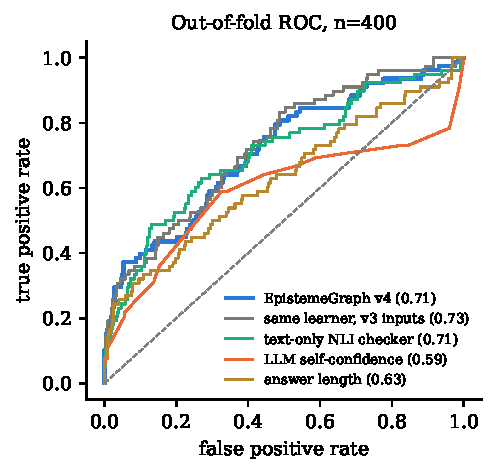
\includegraphics[width=0.82\columnwidth]{figures/roc_cv.pdf}}{}
\caption{Out-of-fold ROC over all labelled answers.}\label{fig:roc}
\end{figure}

\paragraph*{Pool and decisions}
The KG term passes both pool checks ($p=\PoolLRTp$; CV log-loss \PoolCVwith{} versus \PoolCVwithout) with a negative
weight ($b_2=\PoolBkg$), which we read as the verbosity confound again. At $\alpha=0.10$ cross-conformal coverage is
\CVCovTen\% with \CVAbsTen\% abstention and \CVSelTen\% selective accuracy (\cref{tab:conformal}); at $\alpha=0.20$
abstention falls to \CVAbsTwenty\%. On the pre-specified test split ($n=\NTest$) the champion (\Champion) reaches
AUROC \TestAUC{} with coverage \Coverage\%. The full study cost \$\CostRun.

\TableConformal

\section{Discussion and Conclusion}
Label definition and noise set the ceiling: two judges of one family agree moderately and a judge of another family
disagrees systematically, so every metric here should be read against judge agreement and the majority baseline. On a
small KG, claim-level NLI and the model's confidence carry most of the signal; denser graphs are the natural test of
whether geometry matters more. Three papers, one audited model and \NLabelled{} answers limit external validity, and
the conformal guarantee assumes exchangeable calibration and use. EpistemeGraph treats hallucination auditing as
calibrated measurement of a measured reference, and ranks answers far better than the audited model's own confidence.
An extended version with all derivations, ablations and the tournament is in the repository.

\bibliographystyle{IEEEtran}
\bibliography{references}

\end{document}
